\documentclass[11pt]{article}
\usepackage[final]{acl}
\usepackage{latexsym}
\usepackage{amsmath}
\usepackage{booktabs}
\usepackage{graphicx}
\usepackage{xcolor}
\usepackage{url}
\usepackage{tikz}
\usetikzlibrary{positioning, arrows.meta, shapes.geometric, fit, calc, backgrounds}

% Shrink verbatim so shell snippets fit a single ACL column without overflowing
\makeatletter
\renewcommand{\verbatim@font}{\normalfont\ttfamily\footnotesize}
\makeatother
\setlength{\emergencystretch}{6em}

\definecolor{ink}{RGB}{24,31,42}
\definecolor{muted}{RGB}{92,105,122}
\definecolor{rline}{RGB}{205,213,224}
\definecolor{red}{RGB}{176,42,55}
\definecolor{gold}{RGB}{220,158,28}
\definecolor{teal}{RGB}{15,118,110}
\definecolor{blue}{RGB}{37,99,235}
\definecolor{green}{RGB}{22,163,74}
\definecolor{orange}{RGB}{234,88,12}
\definecolor{purple}{RGB}{124,58,237}
\definecolor{soft}{RGB}{246,248,251}
\definecolor{warmsoft}{RGB}{255,246,230}
\definecolor{coolsoft}{RGB}{232,246,240}

\tikzset{
  block/.style    ={rectangle, rounded corners=2pt, draw=rline, fill=soft,
                    inner sep=4pt, minimum height=22pt, font=\small, align=center},
  hostblock/.style={block, fill=warmsoft, draw=orange},
  encblock/.style ={block, fill=coolsoft, draw=green},
  awsblock/.style ={block, fill=soft, draw=rline},
  arr/.style      ={->, >={Stealth[length=2.2mm]}, thick, color=ink},
  thinarr/.style  ={->, >={Stealth[length=1.8mm]}, semithick, color=muted},
  zonelabel/.style={font=\scriptsize\bfseries, color=muted, anchor=north west},
  msglabel/.style ={font=\scriptsize, fill=white, inner sep=1.2pt, align=center},
  notelabel/.style={font=\scriptsize, color=muted, fill=white, inner sep=1pt, align=center},
}

\title{MedSeal: Confidential Medical Record Processing on AWS Nitro Enclaves with Attested Key Release and Infrastructure-Bound PCR Pinning}

\author{Sukeerth Kolakaluri}

\begin{document}
\maketitle

\begin{abstract}
We present \emph{MedSeal}, a confidential-computing system in which
medical records are processed inside an AWS Nitro Enclave whose code
identity (PCR0/1/2) is bound into the AWS KMS key policy as a
recipient-attestation condition, with the policy gate itself enforced
declaratively in Terraform. The EC2 host, the gateway process, the
AWS network plane, and any insider with host root cannot read patient
data. The main contribution is the end-to-end trust pipeline:
client-side envelope encryption, enclave-only plaintext processing,
NSM attestation, PCR-pinned KMS key release, and Terraform-enforced
deployment gates. We implement PHI de-identification and ICD-10
classification as a concrete medical processing task, then validate
the confidentiality claim empirically: a 189\,KB \texttt{tcpdump}
capture across three live production-path requests contains 404
packets, zero plaintext PHI canaries, and visible TLS SNI only for KMS
and the S3 result bucket.
\end{abstract}

\section{Problem Definition}

Standard cloud security protects data at rest (storage encryption)
and in transit (TLS), but not data \emph{in use}: the moment a CPU
processes a record, plaintext exists in registers and host RAM,
where the cloud provider, host operating system, hypervisor admin,
or any attacker with sufficient privilege can read it. This is the
problem the field of confidential computing addresses
\cite{cccsurvey,sgxexplained}.

\paragraph{Scope.} MedSeal solves a narrow but high-value instance:
confidential PHI de-identification \cite{hhsdeid} and ICD-10
classification \cite{icd10} of medical records, where neither the
cloud provider, the host OS, the gateway process, nor any insider
with EC2 root can read the data, even briefly.

\paragraph{Project category.} Relative to the project options,
MedSeal primarily fits trusted execution environment technology and
privacy-preserving software for AWS. It applies AWS Nitro Enclaves,
KMS recipient attestation, IAM, encrypted storage, and Terraform to a
deployed cloud application that processes sensitive data under
hardware-backed isolation.

\paragraph{What is the contribution.} \emph{MedSeal contributes a
working confidential-processing platform for medical records: a
client-side encryption contract, a Nitro Enclave execution boundary,
NSM-backed remote attestation, PCR-pinned KMS key release, and
infrastructure-as-code checks that make the trust chain reproducible.
The included de-identification and ICD-10 pipeline is the medical task
used to exercise that platform; it is intentionally not presented as a
novel NLP model.}

\paragraph{System model and assumptions.}
We trust AWS Nitro hardware and the Nitro Hypervisor
\cite{nitrosystem}; AWS KMS as a service \cite{kmsattested,
kmsenclaves}; the doctor's client device with respect to its own
records; and standard cryptographic primitives: AES-256-GCM
\cite{nistgcm}, RSA-2048 with OAEP-SHA-256 \cite{rfc8017}, SHA-384,
and the COSE\_Sign1 signature on Nitro attestation documents
\cite{rfc9052}.
We do \textbf{not} trust the EC2 host operating system, anything
else running on the host, anyone with EC2 root, the AWS network
plane, AWS employees with infrastructure access (apart from the
hardware itself), or attackers who reach the host through a
software vulnerability. Side-channel CPU attacks, denial of
service, and compromise of AWS at the hardware-vendor level are out
of scope.

\paragraph{Design goals.}
\begin{itemize}\setlength{\itemsep}{1pt}
    \item \textbf{Processing confidentiality:} plaintext PHI exists
    only inside enclave RAM, only for the duration of a request.
    \item \textbf{Verifiable enclave identity:} the recipient of any
    decryption key is the exact code measured at build time.
    \item \textbf{Policy-level enforcement:} the gate is enforced by
    the KMS key policy and a Terraform precondition, not by
    application code; misconfigured deploys fail closed.
    \item \textbf{Reproducible IaC:} a clean account can be brought
    from zero to a verified deployment via Terraform
    \cite{terraform}.
    \item \textbf{Empirical proof:} the confidentiality claim must
    be demonstrable through live traffic capture, not architectural
    argument alone.
\end{itemize}

\section{Conceptual Design}

MedSeal is organized into three trust zones (untrusted client, a
mixed-trust EC2 host that contains both an untrusted gateway and a
trusted enclave, and the AWS service plane) coordinated through a
three-key envelope-encryption protocol. Figure~\ref{fig:arch} shows
the runtime architecture, Figure~\ref{fig:trust} the trust chain,
Figure~\ref{fig:flow} the end-to-end interaction, and
Figure~\ref{fig:pipe} the deployment pipeline that pins the
enclave's identity into the KMS policy.

\begin{figure*}[t]
\centering
\resizebox{0.94\linewidth}{!}{%
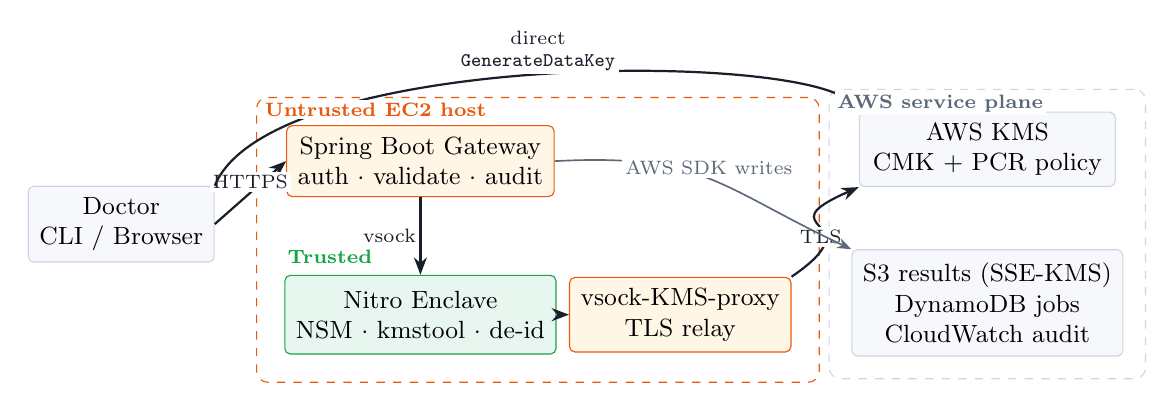
\begin{tikzpicture}[x=1cm, y=1cm]
\node[block, minimum width=2.3cm, minimum height=0.9cm] (client) at (0, 0.05)
  {Doctor\\CLI / Browser};

\node[hostblock, minimum width=3.35cm, minimum height=0.9cm] (gw) at (3.8, 0.85)
  {Spring Boot Gateway\\auth $\cdot$ validate $\cdot$ audit};
\node[encblock, minimum width=3.35cm, minimum height=1.0cm] (enc) at (3.8, -1.10)
  {Nitro Enclave\\NSM $\cdot$ kmstool $\cdot$ de-id};
\node[hostblock, minimum width=2.75cm, minimum height=0.9cm] (proxy) at (7.1, -1.10)
  {vsock-KMS-proxy\\TLS relay};

\node[awsblock, minimum width=3.25cm, minimum height=0.9cm] (kms) at (11.0, 1.00)
  {AWS KMS\\CMK + PCR policy};
\node[awsblock, minimum width=3.25cm, minimum height=1.35cm] (data) at (11.0, -0.95)
  {S3 results (SSE-KMS)\\DynamoDB jobs\\CloudWatch audit};

\draw[arr] (client.east) -- node[msglabel, above]{HTTPS} (gw.west);
\draw[arr] (client.north east) .. controls (1.9,2.25) and (8.7,2.25) ..
  node[msglabel, above]{direct\\\texttt{GenerateDataKey}} (kms.north west);
\draw[arr] (gw.south) -- node[msglabel, left]{vsock} (enc.north);
\draw[arr] (enc.east) -- (proxy.west);
\draw[arr] (proxy.north east) .. controls +(1.1cm,0.75cm) and +(-1.25cm,-0.55cm) ..
  node[msglabel, below]{TLS} (kms.south west);
\draw[thinarr] (gw.east) .. controls +(1.9cm,0.1cm) and +(-1.7cm,0.8cm) ..
  node[msglabel, above]{AWS SDK writes} (data.north west);

\begin{pgfonlayer}{background}
  \node[draw=orange, dashed, fit=(gw)(proxy)(enc), inner sep=10pt, rounded corners=4pt] (zone) {};
  \node[draw=rline, dashed, fit=(kms)(data), inner sep=8pt, rounded corners=4pt] (awszone) {};
\end{pgfonlayer}
\node[zonelabel, color=orange, fill=white, inner sep=1pt] at ($(zone.north west)+(2pt,-1pt)$)
  {Untrusted EC2 host};
\node[zonelabel, color=green, fill=white, inner sep=1pt, anchor=south west] at ($(enc.north west)+(0pt,3pt)$)
  {Trusted};
\node[zonelabel, fill=white, inner sep=1pt] at ($(awszone.north west)+(2pt,-1pt)$)
  {AWS service plane};
\end{tikzpicture}}
\caption{Runtime architecture. The dashed orange box is the
untrusted EC2 host; the green Nitro Enclave inside it is the only
component that ever holds plaintext PHI. The enclave reaches KMS
through the on-host \texttt{vsock-KMS-proxy} because it has no NIC.}
\label{fig:arch}
\end{figure*}

\subsection{Components, in one paragraph each}

\textbf{Client.} A Python CLI or a React browser. Obtains a
per-request Data Key (\S\ref{sec:keys}) directly from KMS
\cite{kmsguide} using scoped client credentials, encrypts the record
locally, wipes the plaintext key buffer, and ships only ciphertext,
IV, tag, and the KMS-wrapped Data Key. The gateway never exposes or
handles a data-key-generation API.

\textbf{Spring Boot gateway} \cite{springboot}. Untrusted. Performs
JWT authentication \cite{springsec}, format validation
(IV $=$ 12 B, tag $=$ 16 B, KMS-key-ARN allow-list, raw-32-byte
``smell test''), DynamoDB job tracking \cite{ddb}, structured
audit, and forwards the encrypted payload to the enclave over
\texttt{AF\_VSOCK}.

\textbf{vsock-KMS-proxy.} A \texttt{systemd} unit running AWS's
\texttt{vsock-proxy} \cite{nitrocli}; forwards
\texttt{AF\_VSOCK} traffic to
\texttt{kms.us-east-1.amazonaws.com:443}. Sees TLS records but
cannot decrypt them.

\textbf{Nitro enclave application.} Python 3.11 in an AWS Nitro
Enclave \cite{nitroug}; no NIC, no disk, no shell. Produces a
COSE\_Sign1 attestation via \texttt{/dev/nsm}, performs the
attested KMS Decrypt through \texttt{kmstool-enclave-cli}
\cite{nitrosdk}, runs spaCy de-id \cite{spacy} and ICD-10
classification \cite{icd10}, then re-encrypts the result.

\textbf{AWS service plane.} A KMS CMK \cite{kmsguide} carrying the
recipient-attestation policy; an S3 bucket
(SSE-KMS \cite{s3ssekms}, public-access blocked, deny-non-TLS) for
encrypted results; a DynamoDB table for job state with PITR and TTL
\cite{ddb}; CloudWatch Logs for audit.

\subsection{Three legs of trust}

The trust model rests on three independent primitives whose
composition is strictly stronger than any one of them:

\begin{enumerate}\setlength{\itemsep}{1pt}
    \item \textbf{Hardware isolation.} The Nitro Hypervisor places
    the enclave in a separate VM whose RAM and CPU state are
    inaccessible to the parent EC2 host's OS, even with root
    \cite{nitrosystem}. No NIC, no disk, no debugger.
    \item \textbf{Remote attestation.} The Nitro Secure Module (NSM)
    at \texttt{/dev/nsm} produces a CBOR-encoded \cite{rfc8949}
    attestation document signed in COSE\_Sign1 format
    \cite{rfc9052} containing PCR0/1/2 (SHA-384 hashes of the EIF,
    kernel, application), an enclave-supplied ephemeral public key,
    a nonce, and a timestamp.
    \item \textbf{Key-release policy.} The KMS key policy contains
    recipient-attestation conditions for PCR0, PCR1, and PCR2
    \cite{kmsattested,kmsenclaves} for both Decrypt and
    GenerateDataKey. AWS validates the COSE signature and the PCRs
    before encrypting the data key into a CMS \texttt{EnvelopedData}
    \cite{rfc5652} addressed to the enclave's ephemeral public key.
\end{enumerate}

\subsection{Three-key envelope encryption}\label{sec:keys}

Each request uses three keys, each with a single role
(Table~\ref{tab:keys}).

\begin{table}[t]
\small
\setlength{\tabcolsep}{4pt}
\begin{tabular}{p{0.20\linewidth} p{0.32\linewidth} p{0.36\linewidth}}
\toprule
\textbf{Key} & \textbf{Purpose} & \textbf{Lifetime / location} \\
\midrule
Master Key (CMK) & Wraps and unwraps Data Keys; carries the policy. & Forever, inside KMS HSM. \\
Data Key (DEK) & AES-256-GCM encryption of the record. & Per-request; client RAM and enclave RAM, then wiped. \\
Ephemeral RSA-2048 & Wraps the KMS reply so the host cannot snoop the DEK in flight. & Per-request; only inside enclave RAM. \\
\bottomrule
\end{tabular}
\caption{The three keys used per MedSeal request.}
\label{tab:keys}
\end{table}

The cryptographic invariant is the standard envelope identity, with
attested wrapping for the KMS reply:
\begin{align*}
C &= \mathrm{AES\text{-}GCM}_{DEK}(P, IV, tag),\\
W &= \mathrm{Enc}_{CMK}(DEK),\\
R &= \mathrm{CMS}_{E_{\mathrm{pub}}}(DEK).
\end{align*}
Here $P$ is the patient record, $C$ is the encrypted record, $W$ is
the KMS-wrapped Data Key, and $R$ is the KMS
\texttt{CiphertextForRecipient}. The final line uses
RSAES-OAEP-SHA-256 \cite{rfc8017} as the key-encryption algorithm and
AES-256-GCM as the content-encryption algorithm. The KMS reply is
computed only when the attestation passes the PCR conditions, and is
encrypted to $E_{\mathrm{pub}}$ so that an attacker on the
vsock-proxy path sees only opaque CMS bytes.

\begin{figure*}[t]
\centering
\resizebox{0.92\linewidth}{!}{%
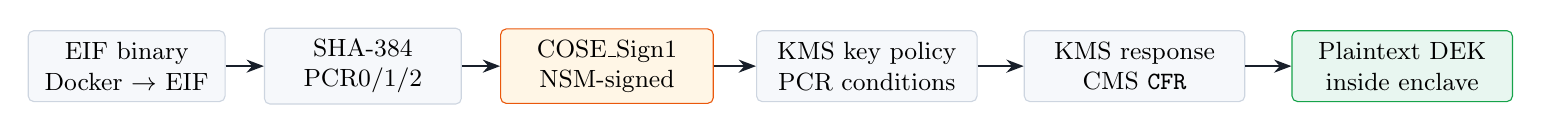
\begin{tikzpicture}[x=1cm, y=1cm]
\node[block, fill=soft, minimum width=2.5cm, minimum height=0.9cm] (eif) at (0,0) {EIF binary\\Docker $\to$ EIF};
\node[block, fill=soft, minimum width=2.5cm, minimum height=0.9cm] (pcr) at (3.0,0) {SHA-384\\PCR0/1/2};
\node[block, fill=warmsoft, draw=orange, minimum width=2.7cm, minimum height=0.9cm] (att) at (6.1,0) {COSE\_Sign1\\NSM-signed};
\node[block, fill=soft, minimum width=2.8cm, minimum height=0.9cm] (pol) at (9.4,0) {KMS key policy\\PCR conditions};
\node[block, fill=soft, minimum width=2.8cm, minimum height=0.9cm] (rel) at (12.8,0) {KMS response\\CMS \texttt{CFR}};
\node[block, fill=coolsoft, draw=green, minimum width=2.8cm, minimum height=0.9cm] (dek) at (16.2,0) {Plaintext DEK\\inside enclave};
\draw[arr] (eif) -- (pcr);
\draw[arr] (pcr) -- (att);
\draw[arr] (att) -- (pol);
\draw[arr] (pol) -- (rel);
\draw[arr] (rel) -- (dek);
\end{tikzpicture}}
\caption{Trust chain. The EIF's content hash is signed by NSM; KMS
verifies the signature and the PCR conditions before re-encrypting
the data key to the enclave's ephemeral public key. Only the
enclave can complete the final unwrap.}
\label{fig:trust}
\end{figure*}

\begin{figure*}[t]
\centering
\resizebox{0.98\linewidth}{!}{%
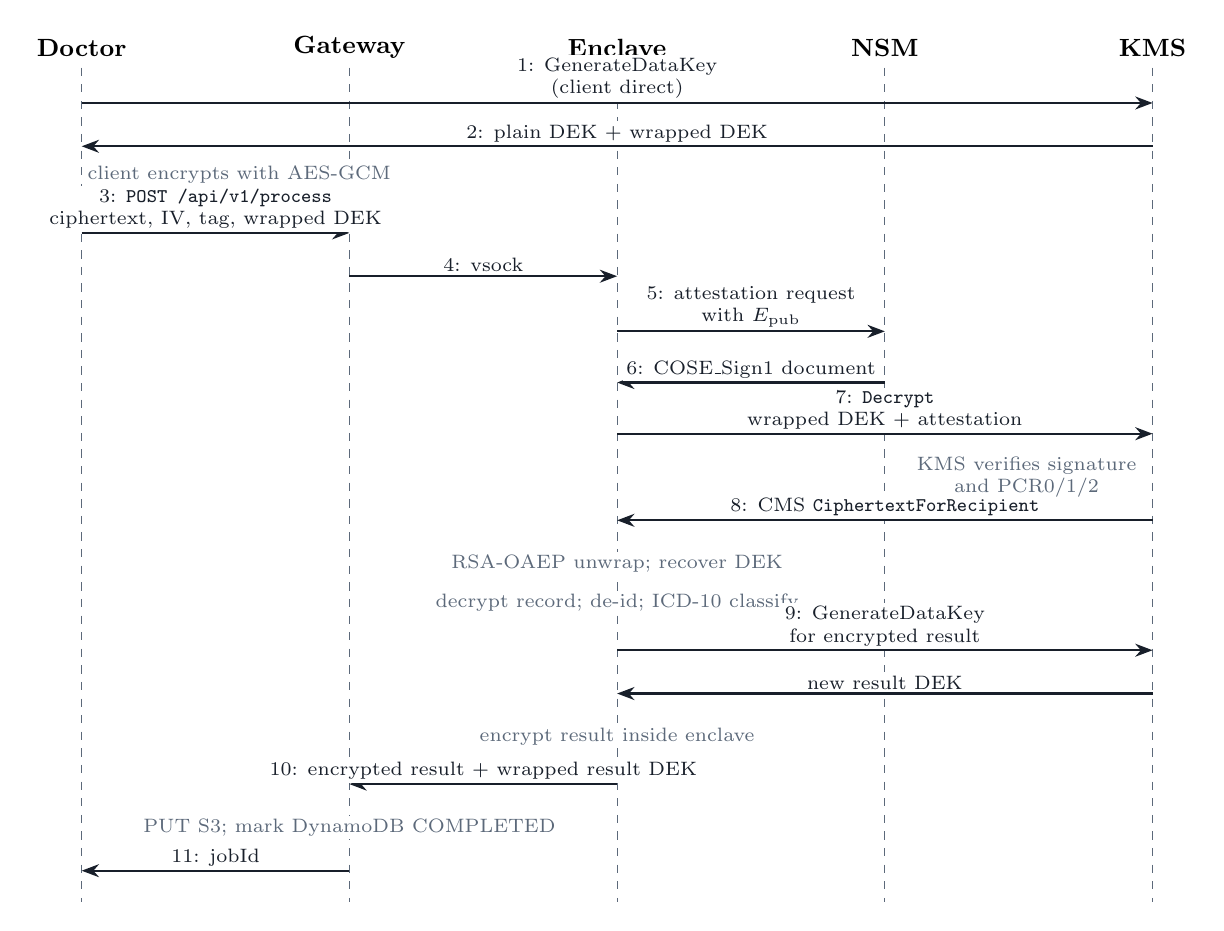
\begin{tikzpicture}[x=1cm, y=1cm]
\foreach \x/\name in {0/Doctor, 3.4/Gateway, 6.8/Enclave, 10.2/NSM, 13.6/KMS} {
  \node[font=\small\bfseries] (top\name) at (\x,0) {\name};
  \draw[color=muted, dashed] (\x,-0.25) -- (\x,-10.85);
}
\draw[arr] (0,-0.7)  -- node[msglabel, above]{1: GenerateDataKey\\(client direct)} (13.6,-0.7);
\draw[arr] (13.6,-1.25) -- node[msglabel, above]{2: plain DEK + wrapped DEK} (0,-1.25);
\node[notelabel] at (2.0,-1.75) {client encrypts with AES-GCM\\and wipes the plain DEK};
\draw[arr] (0,-2.35) -- node[msglabel, above]{3: \texttt{POST /api/v1/process}\\ciphertext, IV, tag, wrapped DEK} (3.4,-2.35);
\draw[arr] (3.4,-2.9)  -- node[msglabel, above]{4: vsock} (6.8,-2.9);
\draw[arr] (6.8,-3.6)  -- node[msglabel, above]{5: attestation request\\with $E_{\mathrm{pub}}$} (10.2,-3.6);
\draw[arr] (10.2,-4.25) -- node[msglabel, above]{6: COSE\_Sign1 document} (6.8,-4.25);
\draw[arr] (6.8,-4.9)  -- node[msglabel, above]{7: \texttt{Decrypt}\\wrapped DEK + attestation} (13.6,-4.9);
\node[notelabel] at (12.0,-5.45) {KMS verifies signature\\and PCR0/1/2};
\draw[arr] (13.6,-6.0) -- node[msglabel, above]{8: CMS \texttt{CiphertextForRecipient}} (6.8,-6.0);
\node[notelabel] at (6.8,-6.55) {RSA-OAEP unwrap; recover DEK};
\node[notelabel] at (6.8,-7.05) {decrypt record; de-id; ICD-10 classify};
\draw[arr] (6.8,-7.65) -- node[msglabel, above]{9: GenerateDataKey\\for encrypted result} (13.6,-7.65);
\draw[arr] (13.6,-8.2) -- node[msglabel, above]{new result DEK} (6.8,-8.2);
\node[notelabel] at (6.8,-8.75) {encrypt result inside enclave};
\draw[arr] (6.8,-9.35) -- node[msglabel, above]{10: encrypted result + wrapped result DEK} (3.4,-9.35);
\node[notelabel] at (3.4,-9.9) {PUT S3; mark DynamoDB COMPLETED};
\draw[arr] (3.4,-10.45) -- node[msglabel, above]{11: jobId} (0,-10.45);
\end{tikzpicture}}
\caption{End-to-end interaction for one
\texttt{encrypt-and-process} request. Step~7 is the attested KMS
Decrypt; step~8 returns the data key inside a CMS
\texttt{EnvelopedData} encrypted to the enclave's ephemeral public
key. Plaintext PHI exists in enclave RAM only between the
bracketed steps after step~8.}
\label{fig:flow}
\end{figure*}

\subsection{Algorithmic invariants}

\paragraph{Invariant~1 (No-plaintext-on-host).}
For every request~$r$, the bytes ever held in the parent EC2
host's address space are a subset of $\{$ciphertext $\cup$
wrapped\_DEK $\cup$ TLS-encrypted KMS records $\cup$ attestation
documents $\cup$ AES-GCM IVs and tags$\}$. Plaintext PHI~$P_r$
never appears in this set. Empirically verified
in~\S\ref{sec:netproof}.

\paragraph{Invariant~2 (Code identity binds key release).}
Let $\mathrm{PCR}(E)$ denote the SHA-384 hash triple of an
EIF~$E$. KMS releases $DEK$ only if
$\mathrm{PCR}(E_{\mathrm{running}}) = \mathrm{PCR}(E_{\mathrm{policy}})$,
where $E_{\mathrm{policy}}$ is the EIF whose PCRs were committed by
the most recent Terraform apply (\S\ref{sec:tfflow}).

\paragraph{Invariant~3 (Fail-closed in production).}
Every component reads \texttt{MEDSEAL\_ENV}. When set to
\texttt{production}, the enclave refuses to start with mock
attestation, mock KMS, missing \texttt{/dev/nsm}, or missing
spaCy model; and the gateway refuses to start without TLS, without
a JWT issuer, or with vsock TCP-fallback enabled. There is no
silent fallback path.

\subsection{Deployment as part of the trust chain}\label{sec:tfflow}

The unique design choice is that the trust gate is enforced not only
at runtime but at deploy time. The KMS key policy contains the
expected PCR values as Terraform variables
(\texttt{allowed\_pcr0/1/2}) with no defaults; a
\texttt{lifecycle.precondition} block in
\texttt{infrastructure/modules/kms/main.tf} rejects empty values
and the literal string \texttt{"PLACEHOLDER"}. A code change
produces a new EIF, which produces a new PCR0; the running stack
stops decrypting until \texttt{terraform apply} is re-run with the
new PCRs. Attestation becomes a deploy-time guarantee, not a hope.

The chicken-and-egg between Terraform and PCRs (Terraform wants
PCRs at plan time; PCRs only exist after the EIF is built) is
resolved with a two-phase apply: a bootstrap \texttt{tfvars} of
all-zero PCRs is applied first (which trivially fails closed
because no real EIF will ever match), then replaced with measured
PCRs after the first build. Figure~\ref{fig:pipe}.

\begin{figure*}[t]
\centering
\resizebox{0.92\linewidth}{!}{%
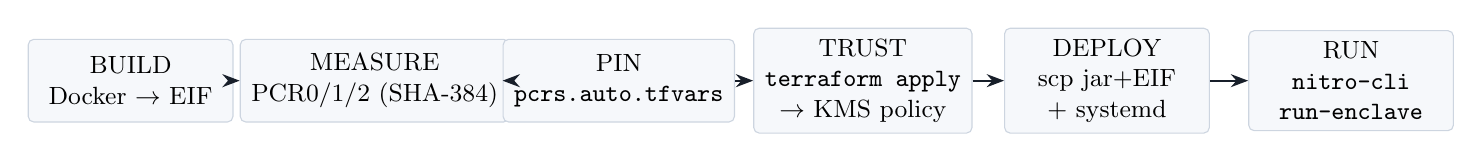
\begin{tikzpicture}[x=1cm, y=1cm, every node/.style={font=\small, align=center}]
\foreach \i/\x/\label in {1/0/{BUILD\\Docker $\to$ EIF},
                          2/3.1/{MEASURE\\PCR0/1/2 (SHA-384)},
                          3/6.2/{PIN\\\texttt{pcrs.auto.tfvars}},
                          4/9.3/{TRUST\\\texttt{terraform apply}\\$\to$ KMS policy},
                          5/12.4/{DEPLOY\\scp jar+EIF\\+ systemd},
                          6/15.5/{RUN\\\texttt{nitro-cli}\\\texttt{run-enclave}}} {
  \node[block, fill=soft, minimum width=2.6cm, minimum height=1.05cm] (s\i) at (\x,0) {\label};
}
\foreach \a/\b in {1/2, 2/3, 3/4, 4/5, 5/6} {
  \draw[arr] (s\a) -- (s\b);
}
\end{tikzpicture}}
\caption{Deployment pipeline. The PIN/TRUST steps couple the EIF's
content hash into the KMS policy, making attestation a deploy-time
property.}
\label{fig:pipe}
\end{figure*}

\section{Implementation Details}

The implementation comprises a Python enclave application, a Java
Spring Boot gateway, a TypeScript+React browser client, a Python
CLI client, and a six-module Terraform configuration. All on-host
services are run by \texttt{systemd}; the EIF is built with
\texttt{nitro-cli build-enclave} \cite{nitrocli} from a pinned
Docker base image. Total $\approx$\,6{,}000 lines across these
languages, of which roughly half is the enclave and crypto
pipeline. The medical processing code provides a realistic record
workflow so that the confidentiality guarantees can be tested on an
end-to-end task.

\subsection{Enclave application}

The enclave application (\texttt{enclave/src/}) is structured into
five subsystems, kept narrow on purpose so that PCR0 stays
deterministic.

\textbf{Attestation.}
\texttt{nsm\_binding.py} is a vendored \texttt{ctypes} wrapper that
opens \texttt{/dev/nsm}, issues the NSM ioctl, and returns the
CBOR-encoded \cite{rfc8949} \texttt{COSE\_Sign1} document
\cite{rfc9052}. \texttt{NitroAttestationProvider} parses the
response and exposes PCR0/1/2 as hex strings.
\texttt{AttestationService} chooses providers from
\texttt{MEDSEAL\_ENV}; mock providers raise at startup in
production.

\textbf{Crypto.}
\texttt{NitroKmsClient} performs an attested KMS Decrypt by
shelling out to \texttt{kmstool-enclave-cli} \cite{nitrosdk}.
\texttt{cryptography} \cite{pyca} handles AES-256-GCM
\cite{nistgcm} and RSA-2048 \cite{rfc8017}; \texttt{pyasn1} and
\texttt{pyasn1-modules} \cite{pyasn1} parse the CMS
\texttt{EnvelopedData} \cite{rfc5652} returned in
\texttt{CiphertextForRecipient}. The pure-Python CMS unwrap is
retained as a unit-tested fallback; \texttt{kmstool} is the
production path because the enclave has no NIC and \texttt{boto3}
cannot complete a TLS handshake without one (\S\ref{sec:lessons}).
Each request now carries the canonical context
$\{\texttt{jobId},\texttt{principal}\}$: clients pass it as KMS
\texttt{EncryptionContext} and as canonical-JSON AES-GCM AAD, while
the gateway requires \texttt{principal} to equal the authenticated
caller before forwarding the context to the enclave. The enclave then
reuses the same context for KMS Decrypt and result encryption. The
invariant is exact-context equality; a swapped job ID, principal, or
wrapped DEK fails as a gateway validation error, KMS error, or
AES-GCM tag failure.

\textbf{Medical processing.}
\texttt{Deidentifier} runs spaCy \cite{spacy} with
\texttt{en\_core\_web\_sm} layered with regex detectors (SSN, MRN,
phone, dates). \texttt{ICD10Classifier} performs rule-based mapping
with curated keyword patterns \cite{icd10}. Both fail closed in
production. A different clinical model with the same input/output
contract would change PCR0 and require repinning, but it would use the
same attestation and key-release architecture.

\textbf{Transport and self-test.}
\texttt{transport/vsock.py} binds CID 16, port 5000, and dispatches
typed JSON requests (\texttt{type:"health"} vs.
\texttt{type:"process"}). \texttt{main.py}'s startup self-test
verifies NSM availability, kmstool invocability, and an end-to-end
mock attestation before the vsock listener opens; failure aborts
with a non-zero exit code.

\subsection{Spring Boot gateway}

\textbf{Controllers.}
\texttt{ProcessController} exposes
\texttt{POST /api/v1/process},
\texttt{GET /api/v1/jobs},
\texttt{GET /api/v1/jobs/\{id\}}, and
\texttt{GET /api/v1/jobs/\{id\}/result}. The two read endpoints
are owner-bound and return HTTP~404 to non-submitters so existence
is not leaked. There is deliberately no
\texttt{POST /api/v1/datakey}; requests to that path return
HTTP~404 so the gateway cannot become a plaintext data-key oracle.
\texttt{StatusController} returns HTTP~503 if any of
\texttt{nsm\_available}, \texttt{kms\_reachable}, or
\texttt{spacy\_loaded} is false on the enclave's typed health
response, and exposes those dependency flags to the operations
dashboard.

\textbf{Service, security, audit.}
\texttt{EnclaveServiceImpl} is the vsock client.
\texttt{SecurityConfig} is a Spring Security \cite{springsec} JWT
resource server, with a static dev-token profile for local
testing. \texttt{ProductionSecurityGuardrails} refuses to start
the application if production-mode invariants are violated.
\texttt{KmsBlobValidator} rejects 32-byte raw-key smell-test
patterns. \texttt{CloudWatchAuditService} writes structured
records with principal, source IP, KMS key ID, attestation hash,
S3 key, processing time, status, and a per-request correlation ID
from \texttt{RequestCorrelationFilter}.

\subsection{Client and CLI}

The Python CLI \texttt{cli/medseal\_cli.py} provides three
sub-commands (\texttt{encrypt-and-process}, \texttt{status},
\texttt{health}). It always calls KMS directly for
\texttt{GenerateDataKey}; the plaintext data key stays in the client
process and the gateway receives only the KMS \texttt{CiphertextBlob}.
The browser client follows the same direct-KMS contract through the
AWS SDK for JavaScript and uses Web Crypto API for AES-GCM. The
data-key buffer is copied into a fresh \texttt{ArrayBuffer} before
use and both buffers are zeroed afterwards. The React UI includes an
operator dashboard with gateway, enclave, NSM, KMS, and model-health
tiles plus a recent owner-scoped request log backed by
\texttt{GET /api/v1/jobs}.

\subsection{Infrastructure}

Six Terraform modules under \texttt{infrastructure/modules/}
declare the entire stack. \texttt{vpc/} provides a VPC with a
public subnet and a security group with explicit ingress CIDRs.
\texttt{ec2/} declares a c5.xlarge with Nitro support and a
user-data script that installs \texttt{aws-nitro-enclaves-cli},
drops the three \texttt{systemd} units, and configures the Nitro
allocator for 2~vCPU and 4~GiB. \texttt{kms/} carries the policy
gating Decrypt and GenerateDataKey on
\texttt{kms:RecipientAttestation:PCR0/1/2}, plus the
\texttt{lifecycle.precondition} that rejects placeholder PCRs.
\texttt{iam/} grants the EC2 role only S3, DynamoDB, and CloudWatch
permissions; it has no direct KMS cryptographic identity policy. KMS
use by the host role is possible only through the key policy's
attested-enclave condition or through the S3-only
\texttt{kms:ViaService} path for SSE-KMS.
\texttt{s3/} enables versioning, SSE-KMS \cite{s3ssekms},
public-access block, deny-non-TLS by bucket policy, and a 30-day
lifecycle. \texttt{dynamodb/} is a PAY\_PER\_REQUEST table with
PITR, TTL on \texttt{expiresAt}, and an owner/timestamp GSI for
dashboard job history \cite{ddb}. \texttt{observability/} declares
CloudWatch log groups, metric filters for completed jobs, failed jobs,
and Nitro enclave hang-ups, two alarms, and an operations dashboard.
A \texttt{backend.tf} stages an S3 + DynamoDB-locking remote backend
that can be enabled after the bootstrap state bucket exists.
Figure~\ref{fig:tfarch} shows the Terraform-declared AWS resource
graph and the policy edges that make the infrastructure itself part of
the security mechanism.

\begin{figure*}[t]
\centering
\resizebox{0.95\linewidth}{!}{%
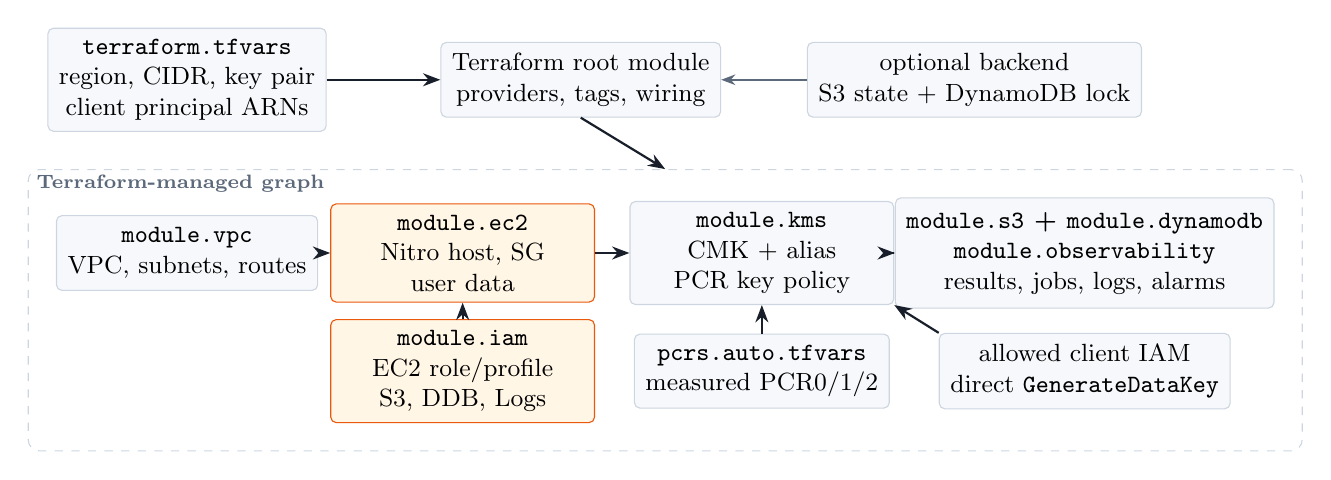
\begin{tikzpicture}[x=1cm, y=1cm, every node/.style={font=\small, align=center}]
\node[block, minimum width=3.4cm, minimum height=0.85cm] (vars) at (0.7, 4.45)
  {\texttt{terraform.tfvars}\\region, CIDR, key pair\\client principal ARNs};
\node[block, minimum width=3.5cm, minimum height=0.85cm] (root) at (5.7, 4.45)
  {Terraform root module\\providers, tags, wiring};
\node[block, minimum width=3.4cm, minimum height=0.85cm] (backend) at (10.7, 4.45)
  {optional backend\\S3 state + DynamoDB lock};

\node[awsblock, minimum width=3.2cm, minimum height=0.95cm] (vpc) at (0.7, 2.25)
  {\textbf{\texttt{module.vpc}}\\VPC, subnets, routes};
\node[hostblock, minimum width=3.35cm, minimum height=0.95cm] (ec2) at (4.2, 2.25)
  {\textbf{\texttt{module.ec2}}\\Nitro host, SG\\user data};
\node[hostblock, minimum width=3.35cm, minimum height=0.95cm] (iam) at (4.2, 0.75)
  {\textbf{\texttt{module.iam}}\\EC2 role/profile\\S3, DDB, Logs};
\node[awsblock, minimum width=3.35cm, minimum height=1.05cm] (kms) at (8.0, 2.25)
  {\textbf{\texttt{module.kms}}\\CMK + alias\\PCR key policy};
\node[awsblock, minimum width=4.1cm, minimum height=1.4cm] (data) at (12.1, 2.25)
  {\textbf{\texttt{module.s3} + \texttt{module.dynamodb}}\\\textbf{\texttt{module.observability}}\\results, jobs, logs, alarms};
\node[block, minimum width=3.15cm, minimum height=0.85cm] (pcrvars) at (8.0, 0.75)
  {\texttt{pcrs.auto.tfvars}\\measured PCR0/1/2};
\node[block, minimum width=3.3cm, minimum height=0.85cm] (clients) at (12.1, 0.75)
  {allowed client IAM\\direct \texttt{GenerateDataKey}};

\begin{pgfonlayer}{background}
  \node[draw=rline, dashed, fit=(vpc)(ec2)(iam)(kms)(data)(pcrvars)(clients), inner sep=10pt, rounded corners=4pt] (modules) {};
\end{pgfonlayer}
\node[zonelabel, fill=white, inner sep=1pt] at ($(modules.north west)+(2pt,-1pt)$)
  {Terraform-managed graph};

\draw[arr] (vars.east) -- (root.west);
\draw[thinarr] (backend.west) -- (root.east);
\draw[arr] (root.south) -- (modules.north);

\draw[arr] (vpc.east) -- (ec2.west);
\draw[arr] (iam.north) -- (ec2.south);
\draw[arr] (ec2.east) -- (kms.west);
\draw[arr] (pcrvars.north) -- (kms.south);
\draw[arr] (clients.north west) -- (kms.south east);
\draw[arr] (kms.east) -- (data.west);
\end{tikzpicture}}
\caption{Terraform-declared AWS architecture. The root module wires
networking, compute, IAM, KMS, S3, DynamoDB, and observability modules. The important
security property is represented by the policy edges: the EC2 role has
storage and audit permissions through IAM, but KMS cryptographic use is
granted by the KMS key policy only for attested enclave requests whose
PCR0/1/2 match the measured EIF, with a separate \texttt{kms:ViaService}
path for S3 SSE-KMS.}
\label{fig:tfarch}
\end{figure*}

\subsection{Operator-facing deployment and customization}

MedSeal is not packaged as a no-code product, but it deliberately
separates the security platform from the demonstration workload. The
AWS architecture is expressed as Terraform modules rather than console
steps; account-specific choices such as region, SSH key, ingress CIDRs,
PCR measurements, bucket/table names, and allowed principals are
provided through \texttt{tfvars}. The deployment scripts then perform
the parts that Terraform cannot know in advance: build the Docker
image into an EIF, read the Nitro PCR measurements, write
\texttt{pcrs.auto.tfvars}, re-apply the KMS policy, copy the gateway
JAR and enclave image to the host, and restart the \texttt{systemd}
services. This turns a security-sensitive manual process into a
repeatable operator workflow.

The practical customization boundary is the enclave workload contract.
A team can change the clinical processor, model files, keyword rules,
or output schema inside \texttt{enclave/src/processing/}; doing so
changes PCR0, so the new EIF must be measured and re-pinned before KMS
will release keys. This is intentional: customization is allowed, but
every customized binary receives a new measured identity. A future
productized version would expose this as a processor plug-in interface
and a small configuration UI for non-security operators; the current
prototype demonstrates the underlying deploy-and-attest mechanism on a
real AWS stack.

\subsection{Empirical verification of confidentiality}\label{sec:netproof}

To turn Invariant~1 from a structural argument into evidence, we
seeded synthetic patient records with high-entropy canary strings
(\texttt{Alicia-CAPTURE-One}, \texttt{Brian-CAPTURE-Two},
\texttt{Carla-CAPTURE-Three}, \texttt{CAPTURE-MRN},
\texttt{asthma and chronic kidney disease}, and three unique phone
numbers). We started \texttt{tcpdump -i any -s 0 -U not port 22} on
the EC2 host and issued three full
\texttt{encrypt-and-process} requests through the direct-KMS client
path. Across 404 packets, 14.1\,s, and a 189\,KB pcap, byte-level
matches for every canary were exactly zero. \texttt{tshark} showed
three authenticated \texttt{POST /api/v1/process} requests carrying
encrypted JSON payloads, plus TLS SNI for
\url{kms.us-east-1.amazonaws.com} and
\url{medseal-results-dev-321052919598.s3.amazonaws.com}. The
gateway-to-enclave channel is \texttt{AF\_VSOCK} and is not visible
on any NIC by construction. We take this as empirical confirmation
of Invariant~1 under the threat model of a passive on-host or
on-VPC sniffer; production TLS adds an outer transport-encryption
layer around the already-encrypted payloads.

\subsection{Live deployment validation}

The most recent validation was run on May~13,~2026 in
\texttt{us-east-1} using the \texttt{medseal} AWS profile. We first
destroyed the prior AWS stack, then recreated it from Terraform, so the
test exercised provisioning rather than only an already-warm
deployment:
\begin{verbatim}
terraform destroy
# Destroy complete! Resources: 35 destroyed.

terraform apply
# Apply complete! Resources: 35 added.
# ec2_public_ip = 44.201.12.205
# kms_key_arn  = ...:key/220c26a5-f599-...
\end{verbatim}
The recreated stack included the Nitro-enabled EC2 host, KMS key, S3
bucket, DynamoDB table, and CloudWatch dashboard. The live KMS key
policy contained the same measured PCR0/1/2 values as
\texttt{infrastructure/pcrs.auto.tfvars}; the running enclave reported
\texttt{RUNNING} on CID~16 with 2~vCPUs and 4~GiB of memory:
\begin{verbatim}
State: RUNNING
EnclaveCID: 16
PCR0: 5ed413...ba973e
PCR1: 4b4d5b...da493
PCR2: 729c0a...ff50
\end{verbatim}
The gateway health endpoint returned all dependency checks as healthy:
\begin{verbatim}
{"status":"UP","nsm":"UP","kms":"UP",
 "gateway":"UP","spacy":"UP","enclave":"UP"}
\end{verbatim}

We then submitted an encrypted medical record through the direct-KMS
CLI path. The client called KMS \texttt{GenerateDataKey} directly with
the canonical $\{\texttt{jobId},\texttt{principal}\}$ encryption
context, encrypted the record locally with AES-GCM using the same
context as AAD, and sent only ciphertext to the gateway. The live job
completed end to end:
\begin{verbatim}
Job ID: 481508b3-acc5-4dd8-9a06-d6a36eb63015
Status: COMPLETED
Processing time: 631ms
Attestation hash: a6d78a3ce0238ead...
\end{verbatim}
The input contained a name, MRN, phone number, date, diabetes mellitus,
and hypertension. The locally decrypted result redacted the PHI fields,
reported six removed PHI entities, and returned ICD-10 matches for
\texttt{I10} and \texttt{E11}. The gateway job API confirmed the
owner-scoped completed job:
\begin{verbatim}
"status": "COMPLETED"
"ownerPrincipal": "dev-user"
"processingTimeMs": 631
\end{verbatim}
The gateway audit log also recorded the completed job with the caller
principal, KMS key ARN, attestation digest, S3 result key, and
correlation ID:
\begin{verbatim}
event=JOB_COMPLETED
jobId=481508b3-acc5-4dd8-9a06-d6a36eb63015
principal=dev-user
attestation_digest=a6d78a3ce0238ead...
s3_key=results/481508b3-.../result.enc
status=COMPLETED
\end{verbatim}

Finally, we ran two negative tests against the live deployment. A
request that supplied \texttt{principal=attacker} while authenticating
as \texttt{dev-user} was rejected by the gateway before enclave
processing:
\begin{verbatim}
HTTPError: 400 Client Error
url: /api/v1/process
\end{verbatim}
A request whose \texttt{jobId} was changed after client-side
encryption reached the enclave but failed closed at KMS because the
KMS \texttt{EncryptionContext} no longer matched the wrapped data key:
\begin{verbatim}
Status: FAILED
Got non-200 answer from KMS: 400
Could not decrypt ciphertext
\end{verbatim}
Together, the successful job and the two negative tests validate both
the confidentiality path and the replay/context-binding path on real
Nitro hardware.

\subsection{Operation complexity}

Let $S$ be the input size in bytes. The enclave performs $O(S)$
symmetric-cryptography work plus $O(1)$ KMS calls (Decrypt for the
input, GenerateDataKey for the result) plus $O(S)$ NLP work in
spaCy. The gateway performs $O(1)$ validation and authentication
plus $O(S)$ I/O. End-to-end latency on a c5.xlarge for a 200-byte
record is 350--670\,ms, dominated by KMS round-trips
($\sim$40\,\%) and S3/DynamoDB ($\sim$25\,\%); spaCy is
$\sim$15\,\% and cryptographic primitives are $\sim$10\,\%.
Latency is linear in $S$, but the constants are dominated by
size-independent round-trips.

\section{User Guide}

\subsection{Prerequisites}
\begin{itemize}\setlength{\itemsep}{1pt}
    \item AWS account with permission to create EC2 (Nitro-capable
    family), KMS, S3, DynamoDB, IAM, VPC.
    \item AWS CLI v2; Terraform $\ge$ 1.5; Java 17; Python 3.11;
    Docker; Nitro Enclaves CLI on the EIF build host.
    \item An imported EC2 SSH key pair, the name of which is
    written into \texttt{infrastructure/terraform.tfvars}.
    \item A PKCS\#12 TLS keystore and either a JWT issuer URI or a
    JWK-set URI for production authentication.
    \item Client IAM principal ARNs permitted to call KMS directly;
    these are listed in \texttt{client\_kms\_principal\_arns}.
\end{itemize}

\subsection{Production deploy (five phases)}
\begin{enumerate}\setlength{\itemsep}{1pt}
    \item \textbf{Configure production variables.}
\begin{verbatim}
cd infrastructure
cp terraform.tfvars.example \
  terraform.tfvars
# Set key_name, ingress CIDR, env="prod",
# s3_force_destroy=false, and client
# KMS principal ARNs.
cd ..
\end{verbatim}
    \item \textbf{Build and measure the EIF.}
\begin{verbatim}
bash scripts/build-enclave.sh
bash scripts/extract-pcrs.sh \
  build/medseal.eif \
  > infrastructure/pcrs.auto.tfvars
\end{verbatim}
    \item \textbf{Apply infrastructure with pinned PCRs.}
\begin{verbatim}
AWS_PROFILE=medseal \
terraform -chdir=infrastructure init
AWS_PROFILE=medseal \
terraform -chdir=infrastructure apply
\end{verbatim}
    \item \textbf{Deploy gateway and start the enclave.}
\begin{verbatim}
mvn -f gateway/pom.xml -B package \
  -DskipTests
export AWS_PROFILE=medseal
export AWS_REGION=us-east-1
export MEDSEAL_ENV=production
export SPRING_PROFILES_ACTIVE=prod
export MEDSEAL_TLS_ENABLED=true
# Also set MEDSEAL_TLS_KEYSTORE_SOURCE,
# MEDSEAL_TLS_KEYSTORE, its password,
# issuer/JWKS, MEDSEAL_DEPLOY_HOST,
# MEDSEAL_SSH_KEY,
# KMS key, S3 bucket, and DDB table.
./scripts/deploy.sh
\end{verbatim}
    \item \textbf{Submit a record from the CLI.}
\begin{verbatim}
export AWS_PROFILE=doctor-prod
export MEDSEAL_TOKEN=<bearer>
.venv/bin/python cli/medseal_cli.py \
  --gateway-url https://<host>:8080 \
  --kms-key-id <key-arn> \
  encrypt-and-process \
    --file path/to/patient.txt \
    --output result.json
\end{verbatim}
\end{enumerate}

\subsection{Verification}
\begin{verbatim}
curl -fsS https://<host>:8080/api/v1/health
# {"status":"UP","enclave":"UP",
#  "gateway":"UP"}

curl -o /dev/null -w '%{http_code}' \
  -X POST https://<host>:8080/api/v1/datakey
# 404

tshark -r medseal_live_capture.pcap \
  -Y tls.handshake.extensions_server_name
grep -a 'PATIENT-CANARY' \
  medseal_live_capture.pcap
# no plaintext PHI matches
\end{verbatim}

\section{Self Evaluation}

We evaluate against the goals of \S1.

\paragraph{Processing confidentiality.} \emph{Met.} See
\S\ref{sec:netproof}: zero plaintext PHI on the wire across three
live requests.

\paragraph{Verifiable enclave identity.} \emph{Met.} The KMS key
policy contains real, non-placeholder PCR0/1/2 produced by
\texttt{nitro-cli build-enclave} and pinned through Terraform.

\paragraph{Policy-level enforcement.} \emph{Met.} PCR variables have
no defaults and a \texttt{lifecycle.precondition} rejects
placeholders; a code change forces a new PCR0 and breaks all
decrypts until the policy is updated.

\paragraph{KMS context and replay binding.} \emph{Met.} Data keys and
payload ciphertexts are bound to $\{\texttt{jobId},
\texttt{principal}\}$ through KMS \texttt{EncryptionContext} and
AES-GCM AAD, and the gateway accepts only contexts whose principal
equals the authenticated caller. Cross-job replay or context tampering
prevents plaintext release by gateway validation, exact-context
mismatch, or AES-GCM tag failure.

\paragraph{Operational observability.} \emph{Met.} The Terraform
observability module declares separate CloudWatch log groups for the
gateway, Nitro, and KMS proxy; metric filters for
\texttt{JOB\_COMPLETED}, \texttt{JOB\_FAILED}, and enclave hang-ups;
alarms on failures and hang-ups; and an operations dashboard.

\paragraph{Reproducible IaC.} \emph{Mostly met.} All application AWS
resources are declared in Terraform. The S3 + DynamoDB-lock remote
backend is staged in \texttt{backend.tf}, but enabling it remains an
account-bootstrap step because Terraform backends must exist before
they can hold state.

\paragraph{Empirical proof of the security claim.} \emph{Met.} The
canary-grep experiment, the live KMS policy with real PCRs, and a
captured \texttt{tcpdump} pcap together form an audit-grade
evidence package. The May~13,~2026 validation additionally exercised
the full deployed stack after a clean destroy/apply cycle, produced a
completed encrypted processing job, confirmed S3/DynamoDB persistence,
verified CloudWatch dashboard availability, and demonstrated two
fail-closed cases: principal mismatch at the gateway and tampered
encryption context at KMS.

\subsection{What was harder than expected}\label{sec:lessons}

The original design used \texttt{boto3.client("kms")} inside the
enclave because that is the reflexive Python pattern. Local unit
tests passed; on real Nitro hardware the enclave exited
$\sim$2\,s after start, because \texttt{boto3} cannot complete a
TLS handshake without a NIC, even with \texttt{vsock-proxy}
running on the host. The fix was an architectural pivot to
\texttt{kmstool-enclave-cli} \cite{nitrosdk}, which uses
\texttt{libnsm} and a vsock-aware C SDK. The lesson:
confidential-computing primitives must be exercised on the actual
TEE; laptop tests are necessary but not sufficient.

\subsection{Open issues}\label{sec:limits}

\textbf{Client credential lifecycle.} The direct-KMS browser path
requires scoped AWS credentials for the client principal. Production
deployments should issue short-lived session credentials through an
identity broker rather than embedding long-lived access keys in the
browser bundle. The CLI path can use standard AWS profile or role
credentials.

\textbf{CloudWatch incident routing.} Terraform now declares log
groups, metric filters, alarms, and a CloudWatch dashboard, and the EC2
bootstrap installs the CloudWatch agent to ship gateway, KMS proxy, and
Nitro logs. The remaining production step is routing alarms to SNS,
PagerDuty, or another incident-management workflow.

\textbf{TLS certificate operations.} The gateway enforces TLS and JWT
configuration in production mode, but certificate provisioning,
rotation, and revocation remain operational tasks outside this
prototype's Terraform modules.

\textbf{Trust assumption.} We trust AWS hardware and the Nitro
Hypervisor. This is identical to every TEE-based system today
\cite{sgxexplained,cccsurvey}.

\section{Contribution}

This project was designed, implemented, deployed, and written up
solely by \textbf{Sukeerth Kolakaluri}. All architectural decisions,
including the
\texttt{kmstool-enclave-cli} pivot of \S\ref{sec:lessons} and the
PCR-pinning Terraform precondition of \S\ref{sec:tfflow}, and
the empirical verification of \S\ref{sec:netproof} were authored,
validated, and signed off by the author.

\begin{thebibliography}{99}

\bibitem[AWS(2026a)]{nitroug}
Amazon Web Services.
\newblock 2026a.
\newblock \emph{AWS Nitro Enclaves User Guide}.
\newblock AWS Documentation.
\newblock \url{https://docs.aws.amazon.com/enclaves/latest/user/}

\bibitem[AWS(2024)]{nitrosystem}
Amazon Web Services.
\newblock 2024.
\newblock \emph{The Security Design of the AWS Nitro System}.
\newblock AWS Whitepaper.

\bibitem[AWS(2026b)]{nitrocli}
Amazon Web Services.
\newblock 2026b.
\newblock \emph{aws-nitro-enclaves-cli}.
\newblock GitHub repository.
\newblock \url{https://github.com/aws/aws-nitro-enclaves-cli}

\bibitem[AWS(2026c)]{nitrosdk}
Amazon Web Services.
\newblock 2026c.
\newblock \emph{aws-nitro-enclaves-sdk-c} (source of
\texttt{kmstool-enclave-cli}).
\newblock GitHub repository.
\newblock \url{https://github.com/aws/aws-nitro-enclaves-sdk-c}

\bibitem[AWS(2026d)]{kmsguide}
Amazon Web Services.
\newblock 2026d.
\newblock \emph{AWS Key Management Service Developer Guide}.

\bibitem[AWS(2026e)]{kmsattested}
Amazon Web Services.
\newblock 2026e.
\newblock \emph{Cryptographic Attestation in AWS KMS}.
\newblock AWS KMS Developer Guide.

\bibitem[AWS(2026f)]{kmsenclaves}
Amazon Web Services.
\newblock 2026f.
\newblock \emph{Using AWS KMS with AWS Nitro Enclaves --
\texttt{kms:RecipientAttestation} policy condition keys}.
\newblock AWS KMS Developer Guide.

\bibitem[Housley(2009)]{rfc5652}
Russ Housley.
\newblock 2009.
\newblock \emph{Cryptographic Message Syntax (CMS)}.
\newblock RFC~5652, IETF.

\bibitem[Bormann and Hoffman(2020)]{rfc8949}
Carsten Bormann and Paul Hoffman.
\newblock 2020.
\newblock \emph{Concise Binary Object Representation (CBOR)}.
\newblock RFC~8949, IETF.

\bibitem[Schaad(2022)]{rfc9052}
Jim Schaad.
\newblock 2022.
\newblock \emph{CBOR Object Signing and Encryption (COSE):
Structures and Process}.
\newblock RFC~9052, IETF.

\bibitem[Moriarty et~al.(2016)]{rfc8017}
Kathleen Moriarty et~al.
\newblock 2016.
\newblock \emph{PKCS \#1: RSA Cryptography Specifications Version 2.2}.
\newblock RFC~8017, IETF.

\bibitem[Dworkin(2007)]{nistgcm}
Morris Dworkin.
\newblock 2007.
\newblock \emph{Recommendation for Block Cipher Modes of Operation:
Galois/Counter Mode (GCM) and GMAC}.
\newblock NIST Special Publication~800-38D.

\bibitem[Costan and Devadas(2016)]{sgxexplained}
Victor Costan and Srinivas Devadas.
\newblock 2016.
\newblock \emph{Intel SGX Explained}.
\newblock IACR Cryptology ePrint Archive 2016/086.

\bibitem[CCC(2023)]{cccsurvey}
Confidential Computing Consortium.
\newblock 2023.
\newblock \emph{A Technical Analysis of Confidential Computing,
Version 1.3}.
\newblock Linux Foundation Whitepaper.

\bibitem[Honnibal and Montani(2017)]{spacy}
Matthew Honnibal and Ines Montani.
\newblock 2017.
\newblock \emph{spaCy 2: Natural language understanding with Bloom
embeddings, convolutional neural networks and incremental parsing}.
\newblock Project documentation, \url{https://spacy.io/}.

\bibitem[Spring(2026a)]{springboot}
Spring Team.
\newblock 2026a.
\newblock \emph{Spring Boot Reference Documentation}.

\bibitem[Spring(2026b)]{springsec}
Spring Team.
\newblock 2026b.
\newblock \emph{Spring Security Reference Documentation}.

\bibitem[PyCA(2026a)]{pyca}
Python Cryptographic Authority.
\newblock 2026a.
\newblock \emph{cryptography: Python library for cryptographic
primitives}.

\bibitem[PyCA(2026b)]{pyasn1}
PyCA.
\newblock 2026b.
\newblock \emph{pyasn1 and pyasn1-modules}.

\bibitem[HashiCorp(2026)]{terraform}
HashiCorp.
\newblock 2026.
\newblock \emph{Terraform Documentation and AWS Provider}.

\bibitem[AWS(2026g)]{s3ssekms}
Amazon Web Services.
\newblock 2026g.
\newblock \emph{Amazon S3: Server-Side Encryption with AWS KMS
keys (SSE-KMS)}.

\bibitem[AWS(2026h)]{ddb}
Amazon Web Services.
\newblock 2026h.
\newblock \emph{Amazon DynamoDB Developer Guide: Time to Live
(TTL) and Point-in-Time Recovery}.

\bibitem[HHS(2012)]{hhsdeid}
U.S. Department of Health and Human Services.
\newblock 2012.
\newblock \emph{Guidance Regarding Methods for De-identification of
Protected Health Information in Accordance with the HIPAA Privacy
Rule}.

\bibitem[WHO(2019)]{icd10}
World Health Organization.
\newblock 2019.
\newblock \emph{International Classification of Diseases, 10th
Revision (ICD-10)}.

\end{thebibliography}

\end{document}
